\documentclass[12pt, a4paper]{article}
\usepackage[top=2cm, bottom=2cm, right=2.5cm, left=2.5cm]{geometry}
\usepackage[utf8]{inputenc}
\usepackage{amsmath, amsfonts, amssymb}
\usepackage{float}
\usepackage{graphicx}
\usepackage{multicol}
\usepackage{xcolor}
\usepackage{xwatermark}
\usepackage{setspace}
% \newwatermark[allpages, angle=45, scale=2.0, color=black!15]{matematicautodidata.com}

\title{Homework}
\begin{document}
\begin{minipage}[c][2cm][c]{2cm}

\includegraphics[height=2cm]{logo.pdf}
\end{minipage}
\begin{minipage}[c][3cm][c]{10cm}
\center
{\scriptsize \textit{Sharif University of Technology}}

% {\scriptsize \textit{Department of Mechanical Engineering}}

\textbf{\normalsize Medical Robotics}

{\small{Assignment \#1}}
\smallskip


\end{minipage}
\begin{minipage}[c][3cm][c]{5cm}
\footnotesize
Date: \today

Dr. Behzadipour


\end{minipage}
\vspace{.5cm}

Mohammad Montazeri \hrulefill \, 404205907

\begin{center}
\textbf{IKP of 6 DoF Manipulator}
\end{center}

Given
\begin{align}
H_6^0 = &\left[\begin{array}{cccc}
& R_6^0 & & \left(\vec{O}_0 \vec{O}_6\right)^0 \\
0 & 0 & 0 & 1
\end{array}\right]_{4 \times 4} \\
\vec{P} = &\left(\vec{O}_0 \vec{O}_6\right)^0 = \left[\begin{array}{c}
    x   \\
    y \\
    z
\end{array}\right] \\
R_6^0 = & \left[\begin{array}{ccc}
    r_{11} & r_{12} & r_{13}  \\
    r_{21} & r_{22} & r_{23}  \\
    r_{31} & r_{32} & r_{33}  
\end{array}\right]
\end{align}

Wanted
\begin{align}
    \theta_1, \theta_2, \cdots, \theta_6
\end{align}

\begin{figure}[htbp]
    \centering
    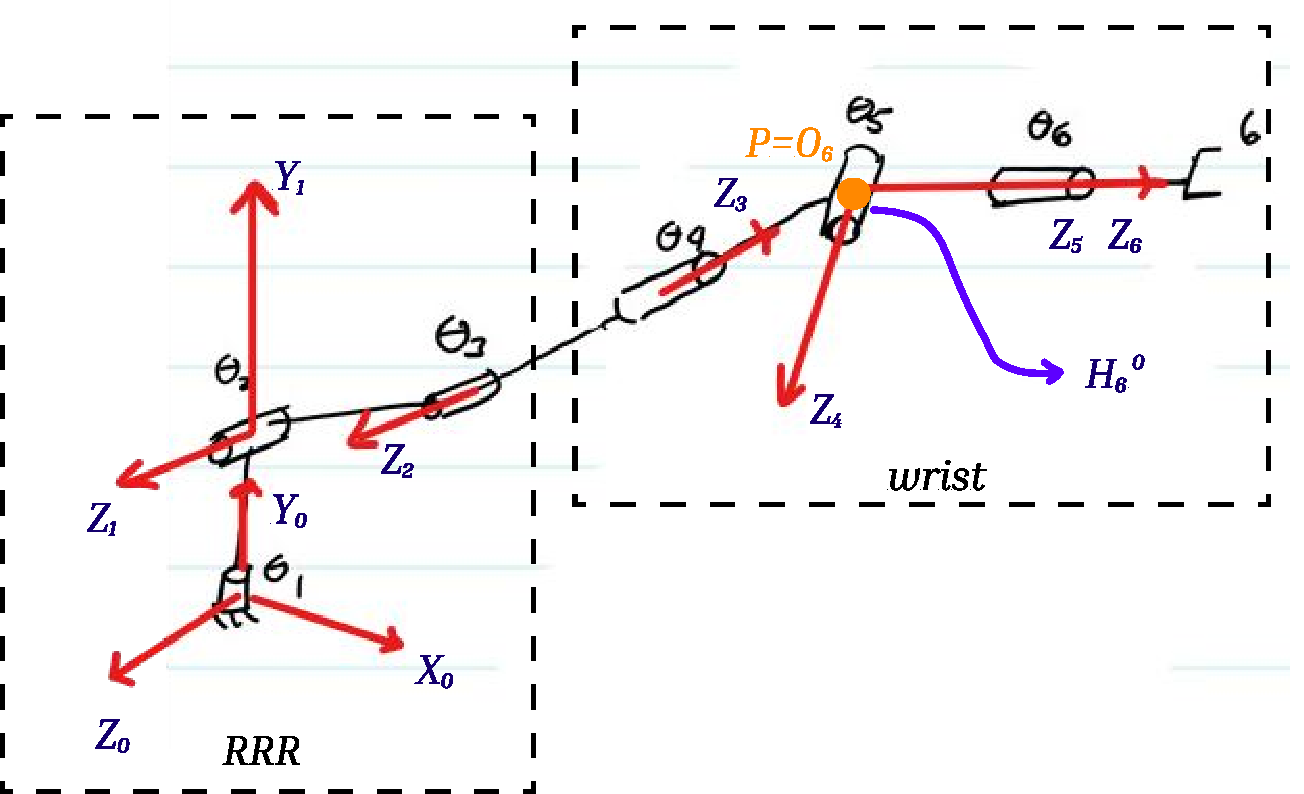
\includegraphics[width=.6\textwidth]{6 DoF.pdf}
    \caption{Schematic view of 6 DoF manipulator with coordinate frames.}
    \label{fig:pic}
\end{figure}

This exercise focuses on a \textbf{decoupled} 6 DoF serial manipulator consisting of an \textit{RRR} and a \textit{Wrist} mechanism. This means the position of the end-effector is controlled using the first 3 links \((\theta_1 \text{ to } \theta_3)\) while the orientation of the end-effector can be adjusted by the next 3 links \((\theta_4 \text{ to } \theta_6)\) independently. Thus, one can solve the IKP of this manipulator by considering the first and second segments separately. Note that for simpler relations, the position of the end effector \((O_6)\) is assumed to be attached to the wrist point \(P\) depicted in figure~\ref{fig:pic}.

According to Lecture 6
\begin{align}
    \theta_1 =& \operatorname{atan}2\left(\frac{x}{\sqrt{x^2+z^2}}, \frac{-z}{\sqrt{x^2+z^2}}\right) \label{eq:pos-start}\\
    \vec{P}_1^{1}=&H_0^{1} \vec{P}_0^0 = \begin{bmatrix}
        X & Y & 0
    \end{bmatrix}^T \\
    [H_0^{1}]=&[{R}_{y_1, -\theta_1}] \, [T_{y_1, -h}] \\
    l_3^\prime = &l_3 + l_4 \\
    l^2=&l_2^2+{l_3^\prime}^2+2 l_2 {l_3^\prime} \cos \theta_3=X^2+Y^2 \\
    \theta_3=&\cos^{-1} \frac{X^2+Y^2-l_2^2-{l_3^\prime}^2}{2 l_2 {l_3^\prime}} \rightarrow \left\{\begin{array}{l}
\theta_3^1 \\
\\
\theta_3^2
\end{array}\right. \\
\theta_2=&\beta-\alpha \\
\Delta O_1 P A \Rightarrow \beta=&\operatorname{atan}2\left(\frac{X}{\sqrt{X^2+Y^2}}, \frac{Y}{\sqrt{X^2+Y^2}}\right) \\
\Delta O_1 P B \Rightarrow \alpha=&\operatorname{atan}2\left(\frac{l_2+{l_3^\prime} \cos \theta_3}{\sqrt{X^2+Y^2}}, \frac{{l_3^\prime} \sin \theta_3}{\sqrt{X^2+Y^2}}\right) \label{eq:pos-end}
\end{align}

Following equations \ref{eq:pos-start} to \ref{eq:pos-end} gives a pair of possible answers for \(\theta_2\) and \(\theta_3\).

\vspace{15pt}

\noindent Now to obtain \((\theta_4 \text{ to } \theta_6)\) we know the orientation from base to end-effector \((R_0^6)\). Also, orientation from base to wrist link (link 3) is \(R_0^3\) (computed from \(\theta_1, \theta_2, \theta_3\)). Thus, wrist orientation would be

\begin{align}
    R_0^3 = & [{R}_{y_0, \theta_1}] \, [{R}_{z_1, \theta_2}] \, [{R}_{z_2, \theta_3}] \\
    R_3^6=&\left(R_0^3\right)^T \cdot R_0^6
\end{align}

Now having \(R_3^6\) one can map it to the rotation matrix corresponding to successive \textit{Z-Y-Z} Euler angles \((\theta_4, \theta_5, \theta_6 = \phi, \theta, \psi)\) .

\begin{align}
R_{(\phi, \theta, \psi)} = \begin{bmatrix}
c_{\phi}c_{\theta}c_{\psi} - s_{\phi}s_{\psi} & -c_{\phi}c_{\theta}s_{\psi} - s_{\phi}c_{\psi} & c_{\phi}s_{\theta} \\
s_{\phi}c_{\theta}c_{\psi} + c_{\phi}s_{\psi} & -s_{\phi}c_{\theta}s_{\psi} + c_{\phi}c_{\psi} & s_{\phi}s_{\theta} \\
-s_{\theta}c_{\psi} & s_{\theta}s_{\psi} & c_{\theta}
\end{bmatrix} = R_3^6
\end{align}

\noindent To find a solution for this problem we break it down into two cases. First, suppose that not both of \(r_{13}\) , \(r_{23}\) are zero. Then from Equation (2.26) we deduce that \(s_{\theta} \neq 0\) , and hence that not both of \(r_{31}\) , \(r_{32}\) are zero. If not both \(r_{13}\) and \(r_{23}\) are zero, then \(r_{33} \neq \pm 1\) , and we have \(c_{\theta} = r_{33}\) , \(s_{\theta} = \pm \sqrt{1 - r_{33}^{2}}\) so

\begin{align}
\theta = \mathrm{Atan2}\left(r_{33},\sqrt{1 - r_{33}^{2}}\right) \label{eq:one}
\end{align}

or

\begin{align}
\theta = \mathrm{Atan2}\left(r_{33}, -\sqrt{1 - r_{33}^{2}}\right) \label{eq:two}
\end{align}

If we choose the value for \(\theta\) given by Equation~\ref{eq:one}, then \(s_{\theta} > 0\) , and

\begin{align}
\begin{array}{rcl}
\phi & = & \mathrm{Atan2}(r_{13}, r_{23}) \\
\psi & = & \mathrm{Atan2}(-r_{31}, r_{32})
\end{array} 
\end{align}

If we choose the value for \(\theta\) given by Equation~\ref{eq:two}, then \(s_{\theta} < 0\) , and

\begin{align}
\begin{array}{rcl}
\phi & = & \mathrm{Atan2}(-r_{13}, -r_{23}) \\
\psi & = & \mathrm{Atan2}(r_{31}, -r_{32})
\end{array}
\end{align}

Thus, there are two solutions depending on the sign chosen for \(\theta\) .

If \(r_{13} = r_{23} = 0\) , then the fact that \(R\) is orthogonal implies that \(r_{33} = \pm 1\) and that \(r_{31} = r_{32} = 0\). Thus, \(R\) has the form

\begin{align}
R = \begin{bmatrix}
r_{11} & r_{12} & 0 \\
r_{21} & r_{22} & 0 \\
0 & 0 & \pm 1
\end{bmatrix}
\end{align}

If \(r_{33} = 1\) , then \(c_{\theta} = 1\) and \(s_{\theta} = 0\) , so that \(\theta = 0\). In this case

\begin{align}
R = 
\begin{bmatrix}
\cos(\phi+\psi) & -\sin(\phi+\psi) & 0 \\
\sin(\phi+\psi) & \cos(\phi+\psi) & 0 \\
0 & 0 & 1
\end{bmatrix}
\end{align}

Thus, the sum \(\phi + \psi\) can be determined as

\begin{align}
\phi + \psi = \mathrm{Atan2}(r_{11}, r_{21}) = \mathrm{Atan2}(r_{11}, -r_{12}) 
\end{align}

If \(r_{33} = -1\) , then \(c_{\theta} = -1\) and \(s_{\theta} = 0\) , so that \(\theta = \pi\). In this case Equation (2.26) becomes

\begin{align}
\begin{bmatrix}
-c_{\phi-\psi} & -s_{\phi-\psi} & 0 \\[4pt]
s_{\phi-\psi} & c_{\phi-\psi} & 0 \\[4pt]
0 & 0 & -1
\end{bmatrix}
=
\begin{bmatrix}
r_{11} & r_{12} & 0 \\
r_{21} & r_{22} & 0 \\
0 & 0 & -1
\end{bmatrix} 
\end{align}

The solution is thus

\begin{align}
\phi - \psi = \mathrm{Atan2}(-r_{11}, -r_{12}) 
\end{align}

As before, there are infinitely many solutions. Note that it was assummed:

\begin{align*}
    \phi \triangleq \theta_4 \\
    \theta \triangleq \theta_5 \\
    \psi \triangleq \theta_6 
\end{align*}

% \begin{enumerate}
% \item
% \item
% \item
% \end{enumerate}

\end{document}